\documentclass[10pt,a4paper]{report}
\usepackage[utf8]{inputenc} 
\usepackage[spanish]{babel}
\usepackage{amsmath}
\usepackage{amsfonts}
\usepackage{amssymb}
\usepackage{graphicx}
\usepackage{multirow}
\usepackage{geometry}
\usepackage{fancyhdr}
\usepackage{hyperref}
\usepackage{url}
\usepackage{natbib}

% Márgenes
\geometry{top=2.5cm, bottom=2.5cm, left=3.0cm, right=2.5cm}

%Cabecera y pie de página
\pagestyle{fancy}
\lhead{\rightmark} 
\chead{} 
\rhead{} 
\lfoot{Antonio Molina García-Retamero}
\cfoot{}
\rfoot{\thepage}

% Interlineado
\renewcommand{\baselinestretch}{1.5}


\author{Antonio Molina García-Retamero}
\title{Optimización de redes neuronales mediante métodos bioinspirados}
\makeindex
\begin{document}
\onecolumn
\maketitle
\pagebreak
\tableofcontents
\pagebreak

\chapter{Introducción}
\section{La propuesta de Trabajo de Fin de Grado}
En este documento se recoge la memoria del trabajo de fin de grado que he realizado y que pretende justificar los valores y facultades adquiridas en el estudio y superación de las competencias recogidas en el Grado en Ingeniería Informática. En estas primeras líneas trataré de exponer el trabajo en términos generales y justificar la elección del mismo y las bondades y problemas del mismo.

\subsection{Justificación y objetivos}
En el proceso de elección del proyecto de fin de grado y de los objetivos a plantear para el desarrollo del mismo, he de indicar que primó mi clara vocación investigadora y es por ello que desde el principio le planteé a mi tutor del proyecto mi deseo de realizar algún tipo de investigación básica, con especial interés es el campo de la inteligencia artificial. Es por eso que este proyecto de fin de grado está generalmente enfocado al desarrollo de una investigación que pueda encontrar una aplicación práctica evidente y que cubra en la medida de lo posible todas las competencias adquiridas durante el grado. Por lo tanto, los objetivos generales que cubren este trabajo serían:
\begin{itemize}
	\item Búsqueda de un problema relativo al campo de estudio sobre el que realizar un proceso investigador con tal de dar solución al problema desde un punto científico-técnico.
	\item Estudio del estado del arte del problema en cuestión.
	\item Planteamiento de soluciones.
	\item Experimentación.
\end{itemize}

La redacción de esta memoria está estructurada haciendo una división entre el trabajo puramente teórico e investigador que será la primera parte de la misma y que tratará de clarificar la metodología de investigación, el planteamiento del problema objeto de estudio y el estudio del estado del arte. En la segunda parte se tratará el diseño y la implementación del banco de pruebas sobre el que realizar el proceso experimentador y se justificará la elección de las tecnologías y metodologías utilizadas. En la tercera parte de esta memoria se detallará la experimentación realizada, se recogerán los resultados y se detallarán las conclusiones del trabajo en su conjunto. 

\chapter{Proceso de investigación}
\section{Planteamiento del problema}
Una vez definido el trabajo y planteados los objetivos de este trabajo fin de grado, el siguiente paso ha sido determinar el problema que se va a tratar dentro del proceso investigador y así tratar de proponer una solución al problema siguiendo una metodología de investigación.
Las redes neuronales artificiales han pretendido, desde su concepción, emular, de alguna manera, el proceso cognitivo que se produce en el cerebro de los mamíferos, siempre a una escala reducida, pero sirviéndose de los mismos principios fundamentales. Sin embargo, el problema del aprendizaje es tradicionalmente objeto de la estadísticas y no de la biología. Las redes neuronales artificiales aplicadas al problema de aprendizaje han sido muy estudiadas como un problema estadístico y existe una muy extensa literatura al respecto, sin embargo, no ha sido hasta años recientes que se está abordando el problema del aprendizaje máquina desde un punto de vista biológico. En los últimos años, la neurocomputación ha adquirido una muy notable importancia dentro del campo del aprendizaje máquina y propone sistemas que realmente pretenden emular a los sistemas biológicos y en los que la posibilidad de llegar a entender quizá un poco más los procesos que dotan a los sistemas biológicos de inteligencia y quizá incluso emular algunas de sus funcionalidades es un campo muy prometedor y cargado de retos ilusionantes.

Partiendo del problema de tratar de emular mecanismos biológicos en los modelos de aprendizaje máquina, mi tutor, Daniel Ruiz, me mostró el trabajo de Diego Andina sobre la aplicación de la metaplasticidad neuronal al perceptrón multicapa (MLP) y me propuso aplicarlo a otro tipo de redes como las RBFN.

\section{El estado del arte}
Dado que partimos de un trabajo en curso, que es la implementación de la metaplasticidad artificial en redes neuronales artificiales, el estudio del estado del arte ha sido un trabajo aurduo que ha requerido de un estudio bastante en profundidad de las diferentes disciplinas bajo las que se contempla el problema que hemos definido y que cubren desde la neurobiología a la estadística y el aprendizaje máquina. Es por esto que me serviré de esta sección primero para demostrar de alguna forma el trabajo realizado en la documentación y adquisición de conocimientos necesarios para comprender el problema y plantear una solución así como para tratar de introducir al lector, de la forma más amena posible, en los conceptos y terminología en que se definen la problemática y la solución propuesta al problema.

El trabajo se inicia con el estudio de lo relativo a la metaplasticidad en las redes neuronales biológicas. Además, he dedicado tiempo a estudiar y entender los modelos estadísticos bajo los que se estudian las redes neuronales artificiales para buscar la forma de aplicar este principio, que es la metaplasticidad artificial, a otros tipos de redes neuronales artificiales más allá, y partiendo, del trabajo que ha desarrollado Diego Andina en las MLP.

Una vez adquiridos los conocimientos necesarios para comprender el problema, se realizará un estudio del estado del arte de las diferentes técnicas de las RBFN con tal de encontrar la forma de aplicar el concepto de metaplasticidad que se da de forma natural en las redes neuronales biológicas.

En las siguientes subsecciones se definirán primero la metaplasticidad en términos biológicos y se expondrá la propuesta de Diego Andina para poder especificar el problema y, partiendo de ahí, plantear la solución propuesta. 

En este punto de la investigación se ha recurrido de nuevo a la bioinspiración tratando de encontrar una perspectiva bajo la que contemplar las RBFN y sobre la que plantear una solución al problema. 

\section{La metaplasticidad en redes biológicas}
Con el término metaplasticidad nos referimos al cambio dependiente de la actividad que modula la plasticidad sináptica en los sistemas neuronales. Estos cambios en la plasticidad pueden ser del tipo LTP\footnote{\textbf{Long-Term Potentiation} es la potenciación de la eficiencia provocada por los eventos más reciente en la señal transmitida entre dos neuronas que se estimulan síncronamente} y LTD\footnote{\textbf{Long-Term Depression} es la reducción de la eficiencia provocada por los evento menos reciente en la señal transmitida entre dos neuronas que se estimulan síncronamente}. Abraham and Bear lo definió de forma sencilla como: \textit{plasticity of synaptic plasticity}, es decir, la plasticidad de la plasticidad sináptica. A diferencia de los mecanismos convencionales de neuromudalación de la plasticidad sináptica en los que son neurotransmisores y hormonas los que inducen cierto grado de LTP y LTD, la metaplasticidad se refiere al cambio que es provocado en un momento dado por lo que comunmente denominamos \textit{primar} la actividad. Es decir, la metaplasticidad se refiere a la inducción en los cambios de los LTP y LTD derivados de la actividad. Reforzando aquellas conexiones sinápticas relativas a las \textit{experiencias} más comunes y deprimiendo aquellas relativas a \textit{experiencias} menos comunes.

Funcionalmente, la metaplasticidad dota a las conexiones sinápticas de la capacidad de integrar señales relativas a la plasticidad a través del tiempo. Además, la metaplasticidad tiene un importante papel como regulador de los umbrales de los LTP y LTD para mantener las conexiones sinápticas en un rango funcional dinámico que evite que estas conexiones se vuelvan demasiado fuertes o demasiado débiles como consecuencia de los mecanismos de plasticidad sináptica convencionales basados en neurotransmisores y hormonas.

\section{Metaplasticidad en redes neuronales artificiales}
El doctor Diego Andina realizó una aproximación a la integración de los mecanismos de metaplasticidad en ..., donde se propone un mecanismo de metaplasticidad artificial (AMP\footnote{Artificial Metaplasticity}) aplicado a las MLP\footnote{Multilayer Perceptron}. En las siguientes líneas trataré de explicar la interpretación que Diego Andina propone sobre la metaplasticidad en el cálculo del error y de la modificación del algorítmo de \textit{backpropagation} propone para la implementación de la AMP en los MLP.

El problema del entrenamiento en cualquier problema de aprendizaje es el de minimizar una función de error ajustando los parámetros del modelo en base a un conjunto de vectores de entrada $x=(x_1,x_2,...,x_n),(x\in\Re^n)$ que conforman el \textit{training set}. En base al criterio de error $E(x)$ que elijamos, el error esperado del sistema será por tanto:
\begin{equation}
	E_M = \int_{\Re^n}E(x)f(x)dx = \int_{\Re^n}e(x)dx
\end{equation} 
Sobre lo que podemos hacer la siguiente transformación:
\begin{equation}
	\label{metaSub1}
	E_M = \int_{\Re^n}\dfrac{e(x)}{f^*_X(x)}f^*_X(x)dx = \varepsilon^*\lbrace\dfrac{e(x)}{f^*_X(x)}\rbrace
\end{equation}
y calcular el error del modelo añadiendo el siguiente estimador:
\begin{equation}
	\label{metaSub2}
	\widehat{E}_M=\dfrac{1}{M}\sum^M_{k=1}\dfrac{e(x^*_k)}{f^*_X(x^*_k)}
\end{equation}
donde $x^*_k,k=1,2,...,M$ son muestras independientes cuya $pdf$ es $f^*_X(x)$. Como se observa, $f^*_X(x)$ es la distribución de probabilidad de la función que tratamos de generalizar con nuestro modelo a través de nuestras muestras de entrenamiento. Por lo tanto, idealmente, 
\begin{equation}
	\label{metaSub3}
	(f^*_X(x))_{opt}=\dfrac{1}{E_M}e(x)
\end{equation}

Lo que se pretende conseguir a través de la introducción de la función subóptima de las ecuaciones \ref{metaSub1} y \ref{metaSub2} es incluir el factor de probabilidad a posteriori de la muestra con tal de provocar un efecto de LTP o LTD en los pesos sinápticos consiguiendo así introducir un mecanismo de metaplasticidad en la red neuronal artificial.
Como se expresa en la ecuación \ref{metaSub3}, la función $f^*_X(x)$ óptima sería la $pdf$ de la señal de entrada de nuestro modelo ($f_X(x)$), lo que es desconocido por nosotros, con lo que, en la práctica, se elige una $f^*_X(x)$ arbitraria tal que $f^*_X(x) \simeq f_X(x)$.

La figura \ref{fig:WeightedTrainEpoch} ilustra como se incorpora el mecanismo de metaplasticidad como un factor de corrección sobre los pesos. Como se observa, esta corrección del error se hace en base a la salida esperada siendo esta, como ya hemos dicho, $f^*_X(x)$.

\begin{figure}[h!]{}
    \centering
    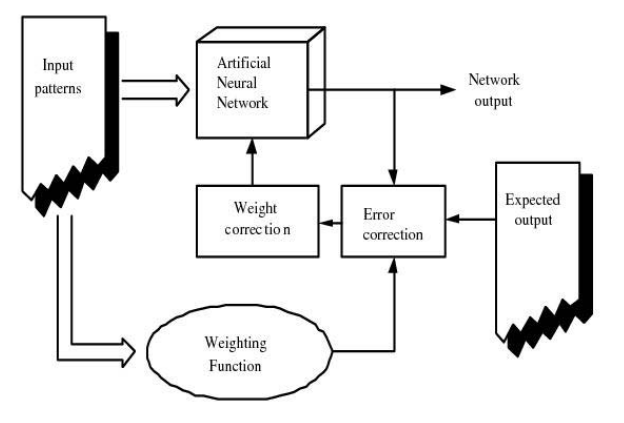
\includegraphics[width=0.6\textwidth]{img/weightingOperation.png}
    \label{fig:WeightedTrainEpoch}
    \caption{Iteración en el entrenamiento de una red neuronal aplicando el mecanismo de metaplasticidad}
\end{figure}


\subsection{Propuesta de implementación de la AMP en las MLP}
En base a esta interpretación que Diego Andina hace de la metaplasticidad en el mismo artículo \citep{Andina2009} se propone la siguiente modificación sobre el algoritmo de \textit{backpropagation} para incluir la función subóptima $f_X(x)$ a los MLP. 
\begin{equation}
	\dfrac{\partial\varepsilon(W)}{\partial w^{(S)}_i} = \dfrac{\partial}{\partial w^{(S)}_i}\left(\dfrac{1}{2}\dfrac{(y-\widehat{y}^{(S)})^2}{f^*_X(x)}\right) = \dfrac{1}{f^*_X(x)}\dfrac{\partial\varepsilon(W)}{\partial w^{(S)}_i}
\end{equation} 
\begin{equation}
	\label{eqErrorLastLayer}
	\delta_j^{(S)} = (y_j - \widehat{y}^{(S)}_j) \cdot \dfrac{f^{'(S)}}{f^*_X(x)}
\end{equation}
siendo s el contador de capas, $s=1,2,...,S$, $j$ e $i$ son el contador de nodos y entradas y $\delta_j^{(S)}$ el error de un nodo $j$ para la capa $s$. Por tanto, la ecuación \ref{eqErrorLastLayer} define el cálculo del error para los nodos de la última capa. Para el resto de capas, el error se propaga siguiendo la forma convencional del \textit{backpropagation}.
En definitiva, lo que se propone es incluir para, cada iteración en el entrenamiento, es ponderar ese peso en un factor que es el siguiente:
\begin{equation}
	w^*(x) = \dfrac{1}{f^*(x)}
\end{equation}
con lo que se consigue acelerar el entrenamiento dando más importancia a los casos menos frecuentes. Esto además es acorde con la teoría de la información en tanto que \textit{los sucesos menos frecuentes contienen más información}.

De todo lo comentado anteriormente, queda patente que una de las claves en la implementación de la metaplasticidad a las redes neuronales es la elección acertada de la función subóptima $f_X(x)$. En el caso concreto de las MLP, para clasificar $L$ clases $H_l$ para $l=0,1,...,L-1$, y basándonos en el teorema de Bayes, obtenemos
\begin{equation}
	\widehat{y}_l \simeq P(H_l/x)=\dfrac{f_X(x/H_l) \cdot P(H_l)}{f_X(x)}
\end{equation}
si asumimos la salida de nuestra red $\widehat{y}_l$ como $P(H_l/x)$, la propia salida de la red neuronal generaliza $f_X(x)$ con lo que esta puede ser utilizada como función subóptima.

De esta forma, Diego Andina obtiene los resultados de la figura \ref{fig:andinaResults} y que representa la media del error para redes con la modificación propuesta (BPW) para un número creciente de operaciones en contraposición con la media del error en redes entrenando con un algorítmo de \textit{backpropagation} tradicional(BP). En este caso, la función de distribución de probabilidad, se ha asumido la siguiente gaussiana
\begin{equation}
	f^*_X(x) = \dfrac{A}{\sqrt{(2\pi)^n} \cdot e^{\dfrac{B}{8} \sum_{i=1}^n{x_i^2}}}
\end{equation}
donde $A$ y $B$ son los parámetros de la gaussiana que en este caso representan los parámetros de la metaplasticidad. En el artículo\citep{Andina2009} se muestra el siguiente ejemplo de como puede mejorar esta propuesta para una entrada concreta en un escenario, se supone, ideal:

\begin{figure}[h!]{}
    \centering
    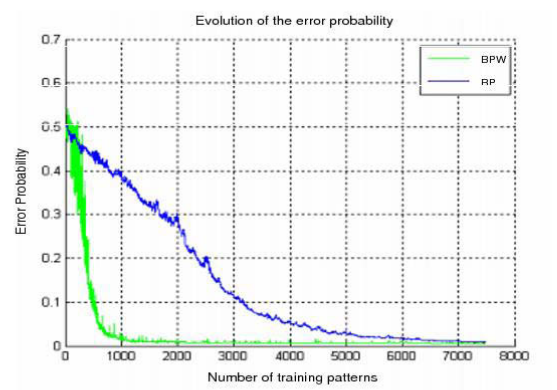
\includegraphics[width=0.6\textwidth]{img/ArticleResults.png}
    \label{fig:andinaResults}
    \caption{Comparación de la evolución del aprendizaje del algorítmo ponderado (BPW) frente al tradicional (BP)}
\end{figure}

\subsubsection{Implementación propia}
Sobre esta propuesta de modificación del algorítmo de \textit{backpropagation} realicé mi propia implementación con tal de poder hacer mi propia experimentación. Esta implementación la basé en el desarrollo de una MLP que realicé para la asignatura de \textit{Razonamiento Automático} en C++. El objetivo de esta implementación era tan solo el de poder experimentar de primera mano, utilizar diferentes funciones subóptimas y diferentes datos de entrenamiento. 
Así, en la siguiente subsección expondré las conclusiones derivadas del estudio y la experimentación de la técnica propuesta por Diego Andina.
 Esta implementación está publicada en el siguiente repositorio de \href{https://github.com/aydevosotros/AMMLP}{GitHub}\footnote{https://github.com/aydevosotros/AMMLP}.

\fbox{Esto creo que se me queda corto, pero tampoco se muy bien que más decir}

\subsubsection{Conclusiones del estudio}
Una vez asimilados los conceptos y habiendo realizado una implementación y haber experimentado primero sobre el conjunto de datos sobre los que se publica el artículo y después con otros conjuntos de datos públicos y típicos en los problemas de aprendizaje máquina y habiendo experimentado con diferentes funciones subótimas, he alcanzado las siguientes conclusiones
\begin{itemize}
	\item Encontrando una función subóptima que se aproxime a la función de distribución de probabilidad de los datos que componen la señal de entrada podemos obtener una gran mejora emulando los procesos LTP y LTD de los sistemas biológicos.
	\item A priori, $f_X(x)$ es desconocida en los problemas de aprendizaje máquina, con lo que escoger una $f^*_X(x)$ subótima apropiada es un problema muy considerable.
	\item La posibilidad de aproximar $f_X(x)$ por la salida de la red neuronal $\widehat{y}_l$ cuando esta está lo suficientemente entrenada como para proveer una aproximación lo suficientemente buena puede ser muy interesante.
\end{itemize}

\section{Metaplasticidad Artificial en RBFN}
En esta sección trataré de expresar la problemática observada en el proceso de encontrar y aplicar algún mecanismo de metaplasticidad artificial aplicado a las redes neuronales con función de activación de base radial (RBFN). Para ello, haré en primer lugar una breve introducción a las RBFN tratando de introducir al lector en las principales características de este tipo de redes para después exponer una primera solución y la problemática encontrada.
\subsection{Definición y características de las RBFN}
Para el estudio de las RBFN, fundamentalmente he estudiado el libro de \textit{Simon Haykin}\cite{haykin99a}. 

\begin{figure}[h!]{}
    \centering
    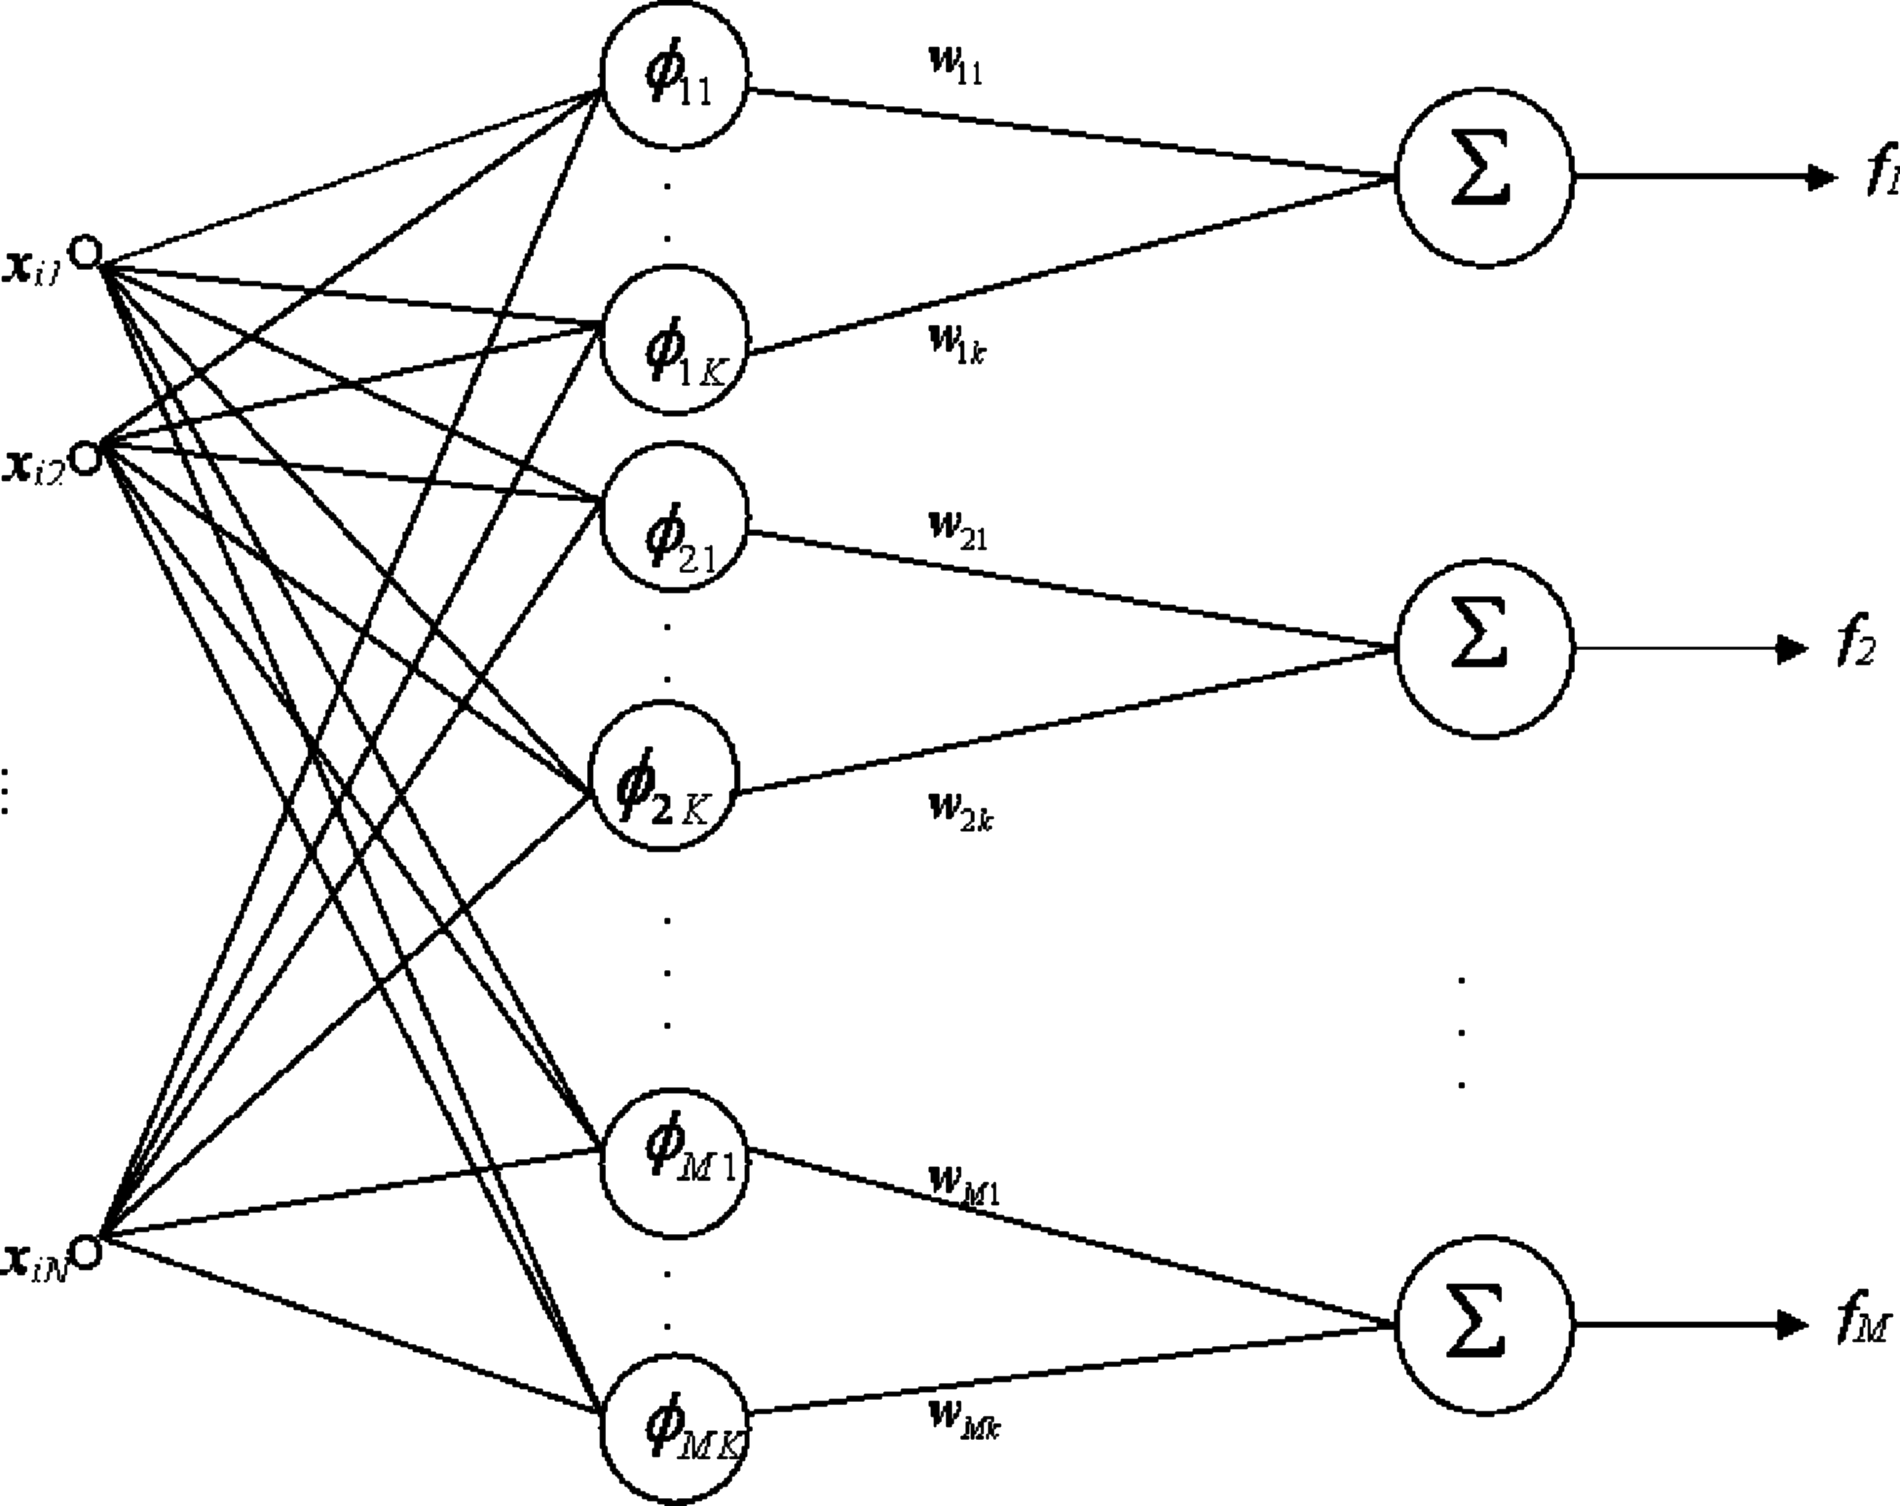
\includegraphics[width=0.6\textwidth]{img/RBFN1.png}
    \label{fig:RBFN1}
    \caption{Arquitectura de las RBFN}
\end{figure}

\subsubsection{Metodologías de entrenamiento}
\subsection{Aplicación directa del estimador de probabilidad}
Una primera implementación de la metaplasticidad en las RBFN podría ser la de incluir la estimación de probabilidad subóptima en la fase de entrenamiento de pesos con tal de ponderarlos de forma similar a, como explicado, Diego Andina propuso para las AMMLP\citep{Andina2009}.

De la misma forma que explicamos anteriormente, 
\begin{equation}
	E_M = \int_{\Re^n}{e(x)dx}
\end{equation}
hacemos igualmente la transformación con tal de incluir el estimador $f^*_X(x)$
\begin{equation}
	\label{metaRBFN1}
	E_M = \int_{\Re^n}\dfrac{e(x)}{f^*_X(x)}f^*_X(x)dx = \varepsilon^*\lbrace\dfrac{e(x)}{f^*_X(x)}\rbrace
\end{equation}
para obtener de nuevo el error del sistema en función del criterio de error que elijamos $e(x^*_k)$ y la función de distribución de probabilidad $f^*_X(x)$
\begin{equation}
	\label{metaRBFN2}
	\widehat{E}_M=\dfrac{1}{M}\sum^M_{k=1}\dfrac{e(x^*_k)}{f^*_X(x^*_k)}
\end{equation}

\subsubsection{Propuesta de implementación}
Para aplicar este nuevo cálculo del error a una RBFN, tan solo hemos de aplicar el criterio de error a la propia red. Si consideramos el criterio de error más típico que es el del cuadrado de la diferencia e incluyéndolo en \ref{metaRBFN2} obtenemos:
\begin{equation}
	\label{metaRBFN3}
	\widehat{E}_M=\dfrac{1}{M}\sum^M_{k=1}\dfrac{(y_k - \overbrace{\left(\sum^M_{j=1}{w_j G(\Vert x^*_k - t_j \Vert_{C_j})}\right)}^{Salida\ de\ la\ RBFN})^2}{f^*_X(x^*_k)}
\end{equation}
que sustituiremos la derivada parcial respecto $w_i$
\begin{equation}
	\dfrac{\partial\varepsilon(n)}{\partial w_i(n)} = \sum^N_{j=1}{\widehat{E}_M(n) G(\Vert x_j - t_i \Vert_{C_i})}
\end{equation}
Por tanto, y en términos del algorítmo general, el entrenamiento de nuestra RBFN solo cambia con respecto a las técnicas de entrenamientos típicas con la única variación de que la función de coste será la definida en \ref{metaRBFN3}
\begin{equation}
	w_i(n+1)=w_i(n) - \eta \dfrac{\partial\varepsilon(n)}{\partial w_i(n)}
\end{equation}

\subsection{Problemática}
Una vez asumido el concepto de metaplasticidad en las redes neuronales biológicas y partiendo de la propuesta de metaplasticidad artificial en las MLP de Diego Andina, estamos en disposición de abordar el problema. 
Como ya se ha expuesto anteriormente y en esencia, la propuesta de Diego Andina se basa en la emulación de los procesos LTP y LTD añadiendo un factor que pondera la derivada parcial en el descenso por gradiente de la muestra con respecto al peso de la conexión sináptica que representa cuan \textit{raro}, en términos de probabilidad, es la muestra respecto a la clase en que se clasifica a posteriori. Esta probabilidad a posteriori se estima por la propia salida de la red neuronal en ese estado del entrenamiento. 

En este punto, queda patente que existe numerosos problemas a la hora de aplicar esta técnica a otro tipo de redes neuronales, en particular en las RBFN. En la figura \ref{fig:RBFN1}, se representa la arquitectura típica de una RBFN.

Un problema fundamental se debe a la salida de la última capa de sendas redes neuronales. Para implementar un mecanismo de metaplasticidad similar al descrito en las AMMLP, se requiere de una estimación de la probabilidad de pertenencia a la clase (cuan \textit{rara} es la muestra) y en las AMMLP la estimamos como la salida de la propia red neuronal. Ya que la neurona de la última capa es una función logística \footnote{Una función logística es una función continua cuya salida $\in [0 1]$. Un ejemplo de función logística típia es \\ $f_{log}(z)=\frac{1}{1+e^{-z}}$}, asumimos ésta como la probabilidad a posteriori de pertenencia a la clase. Por su parte, la salida de una RBFN para el problema de clasificación se calcula como $sign(f(x)=\sum w \phi(x))$. Queda patente que la salida de la RBFN no nos sirve para estimar una probabilidad a posteriori de la muestra.

Sin embargo, la propia naturaleza de las RBFN parece resultar idónea a su vez para experimentar con técnicas. Este \textit{parecer} es una percepción completamente intuitiva, pero existen ciertas características que trataré de explicar a continuación que pueden hacer de estas redes idóneas para representar las redes neuronales biológicas y a la forma en que estas representan la información y que me inspiraron a plantearme el problema en multitud de formas tratando de encontrar la forma de encajar estas características con la naturaleza del aprendizaje y de la metaplasticidad. Estas características son, en líneas generales:

\begin{itemize}
	\item La capa oculta característica de las RBFN está compuesta por \textit{neuronas} cuya función de activación es típicamente una gaussiana en la forma . Estas gaussianas tienen dos parámetros básicos y que son fundamentalmente dependientes de la naturaleza de la señal de entrada y que son un centroide y la varianza.
	\item La capa oculta, a su vez, realiza una transformación no lineal en un espacio basado en la distancia. Esta característica sirve de nexo para el estudio de las RBFN dentro del conjunto de los \textit{Kernel Methods}.
	\item La matriz de covarianza determina el campo receptivo de las funciones de activación de base radial gaussianas.
\end{itemize}

Expuestos los problemas y las caracterísitcas más relevantes en este estudio, continué la investigación buscando técnicas a través de las cuales poder extraer información que pudiera estimar la función de distribución de probabilidad de la señal de entrada. Tal y como hemos visto anteriormente, existen típicamente dos fases de entrenamiento y en la primera de estas se trata de encontrar la posición de los centroides en el espacio de características para las gaussianas de la capa oculta y, en ocasiones, estimar una covarianza para estas gaussianas. Esta primera fase es, por tanto y básicamente, una búsqueda de información sobre la señal de entrada donde tratar de estimar de alguna forma $f_X(x)$ y utilizarlo en la segunda fase de entrenamiento para ponderar los pesos con la función $w^*$ en un descenso por gradiente en busca de minimizar la función de coste de nuestra red.

\section{Ampliación del estado del arte}

\subsection{Tonotopía y Retinotopía}
\subsection{Kernel Methods}
\section{Propuesta de solución}
En base a los trabajos previos, la idea de servirnos de la naturaleza de los datos de nuestro entrenamiento para hacernos una idea a priori de cuan significativa es una muestra y actuar ponderando esa "conexión sináptica" concreta parece encajar de forma especial en el concepto de RBFN debido a la naturaleza de las Funciones de Base Radial. Quiero decir, las Funciones de Base Radial nos proporcionan una transformación no lineal que nos permite encontrar un hiper-plano que en algún espacio multidimensional nuestros datos serán separables. El modelo de las RBFN, como ya hemos comentado, se sirven de un modelo con la forma $f(x)=\sum w \phi(x)$ donde $\phi(x)$ es un función de base radial. Este tipo de funciones pueden ser muy variadas y se ha experimentado con multitud de ideas alrededor de esto sin embargo en los casos más habituales se utiliza una función gaussiana en donde tenemos que inferir tanto la media como los centroides para cada una de las funciones en nuestro conjunto de datos. De esto se deriva un entrenamiento de dos fases en el que en la primera fase inferimos los datos necesarios para calcular la activación de la capa oculta para hacer luego encontrar los parámetros para la transformación lineal sobre la salida de esta capa en una segunda fase de entrenamiento.

Aquí es donde pretendo encontrar y probar diferentes formas de optimizar la segunda fase de entrenamiento sirviéndonos del estudio estadístico que implica la primera fase. Esto es, Cuando en la primera fase de entrenamiento buscamos los centros para nuestras funciones de activación obtenemos información relevante que podemos utilizar para estimar, como hablábamos antes, como considerar una probabilidad de pertenencia a una clase si consideramos el centroide como una clase, etc... Multitud de ideas se pueden considerar y en última instancia lo que se estaría haciendo sería entremezclar de diferentes formas el proceso de aprendizaje no supervisado a priori para influir en el proceso de aprendizaje supervisado de la segunda fase.


\chapter{Implementación}
Con tal de dar soporte al planteamiento teórico que ha sido expuesto en la sección anterior, he desarrollado un \textit{benchmarks} sobre el que realizar la experimentación que sustente la validez (o pruebe la falta de esta) de los algoritmos propuestos. Pese a tener un objeto muy concreto, he tratado de realizar un diseño tan generalista como me fuera posible, tratando de definir y delegar las responsabilidades entre clases y persiguiendo siempre un bajo acoplamiento y una alta cohesión entre estas.
En líneas generales, el software desarrollado ha de cubrir los siguientes objetivos:
\begin{itemize}
	\item Implementar una \textbf{RBFN} configurable tanto en los parámetros propios de la RBFNN (dimensionalidad, parámetros de las gaussianas, etc...) como en los algorítmos de entrenamiento.
	\item Implementar un mecanismo de \textbf{generación/obtención} de los conjuntos de datos:
	\begin{itemize}
		\item Ha de ofrecer la posibilidad de generar datos aleatorios en base a una \textit{fdp} ($f_X(x)$) conocida con tal de facilitarnos la experimentación en nuestro problema en concreto en el que, como se ha discutido ampliamente en secciones anteriores, esta función tiene un papel fundamental.
		\item Además, ha de ofrecer diferentes conjuntos de datos reales con tal de posibilitar la experimentación y comparación de estos algoritmos con el estado del arte del problema.
	\end{itemize}
	\item Implementar un mecanismo que recopile los resultados obtenidos y \textbf{genere un informe} con toda la información necesaria para evaluar estos resultados
\end{itemize}

Una vez especificados los objetivos, en las siguientes subsecciones describiré y justificaré las metodologías escogidas para el desarrollo del software. Además, describiré y justificaré la elección del lenguaje de programación escogido y de las herramientas en las que me he apoyado para el desarrollo. Por último, trataré de ir describiendo los diferentes paquetes que he desarrollado para cubrir cada uno de los requerimientos que se han planteado en forma de objetivos \textit{(RBFN, Generador de datos, Generador de informes)}

El objetivo final del software a desarrollar es el de proveer de un \textit{framework} de desarrollo rápido que fuera lo más general y flexible posible para poder realizar una experimentación lo más rápida y cómoda posible. Es decir, el objetivo último era conseguir un entorno con las siguientes características:
\begin{itemize}
	\item \textbf{Flexible:} 
	\item \textbf{Extensible:}
	\item \textbf{Desarrollo rápido:}
\end{itemize}

De esta forma, la experimentación será un ejercicio dinámico en la que fácilmente cambiar los diferentes parámetros y algoritmos y experimentar sobre diferentes conjuntos de datos. La experimentación, en multitud de ocasiones, se trata de un ejercicio de ensayo-error guiado por un proceso creativo en donde la simplicidad de las herramientas juega un papel muy importante y por lo tanto, el diseño ha tenido como requisito constante exponer un conjunto de objetos sencillos, claros y fáciles de utilizar y que a su vez sean altamente parametrizables y extensibles en su comportamiento.


\section{Metodología de desarrollo}
En cuanto a las metodologías de desarrollo, en fase de diseño, determiné usar diferentes metodologías para afrontar los diferentes problemas y con tal de aprovechar las ventajas que, sobre cada uno de los problemas, estas ofrecen.

Así pues, para implementar la RBFN me serví de un desarrollo basado en Test Driven Development (TDD). Debido a la complejidad de implementación a la susceptibilidad de errores de implementación en los algorítmos, me aproximé al desarrollo de la red neuronal basándome en diferentes pruebas lo suficientemente sencillas para poder precalcular cada uno de los resultados de los algoritmos y garantizar así la correcta implementación. Así mismo, el diseño de la clase vino determinado por las necesidades que surgían al diseñar las pruebas y que, por lo tanto, siguiendo un desarrollo \textit{up-to-bottom}.

Para el desarrollo del generador de datos realicé un Diseño Orientado a Objetos con un enfoque cercano a la Programación Extrema. Esto es, dado que los requisitos para el generador de datos, descritos anteriormente, me permitían hacer un diseño de clases bastante claro ya que los propios requisitos definen la interfaz pública de la clase generadora de datos (\textit{generarDataSet, obtenerX, obtenerY, etc...}).

Por último, para el generador de informes me serví de una combinación de estas. Es decir, partía de un resultado esperado que era el informe y una interfaz pública más o menos clara (\textit{addGrafico, addSection, etc}). Sin embargo en tiempo de desarrollo, las pruebas fueron redefiniendo esta interfaz en base a los requisitos que iban imponiendo las pruebas rediseñando así el modelo en cada \textit{iteración} del desarrollo.

\section{Esquema general del diseño}
Ya que el objetivo fundamental del desarrollo es el de proveer de un entorno de experimentación con los requisitos que se han descrito en la introducción de este capitulo, he decidido plantear el desarrollo como una pequeña librería de clases que me ofrezca clases listas para instanciar y con unos pocos parámetros de configuración me provea de diversas configuraciones (tipo de RBFN, conjunto de datos, etc..) para un experimento. Así, con unas pocas líneas de código debería ser capaz de, obtener una RBFN con o sin metaplasticidad y con los parámetros propios de la red deseados, obtener un conjunto de datos con las características deseadas y realizar tantas pruebas como se quiera. Además la recogida de datos deberá ser asistida por una clase que permitirá la construcción de tablas y gráficos y construirá el código LaTeX requerido para la representación de estos.
Por lo tanto, nuestra librería constará de 3 clases en las que se delegarán las 3 responsabilidades descritas:

(Aquí la imagen de las 3 clases)

\section{Lenguaje y herramientas}
Establecidos los objetivos, metodologías, requisitos y diseño general, me propongo a decidir bajo que entorno construir la librería.
Una primera opción muy recurrida en los entornos investigadores es el uso de \textit{Matlab}. Este entorno muy popular y potente ofrece un numero enorme de algoritmos categorizados, estructurados y fáciles de usar se ha ganado su popularidad en entornos de investigación muy merecidamente ya que en un solo entorno integra todo lo requerido para prácticamente cualquier investigación en cualquier campo. Además cumple perfectamente con los requerimientos que pueda tener para el desarrollo descrito. Sin embargo, este entorno es privativo y de código cerrado. Además, los costes de su licencia son muy considerables, y en tanto me fuera posible, intento siempre utilizar herramientas abiertas.

De entre las alternativas abiertas, existen numerosas (y algunas muy buenas) aproximaciones al entorno \textit{Matlab} como puede ser \textit{octave} para el que existe una gran comunidad y multitud de librerías y módulos para extenederlo a muy diversas áreas. Otra aproximación a este tipo de entornos es la librería para \textit{Python} \textit{SciPy} que aglomera un conjunto de paquetes que abarcan gran parte de los requerimientos comunes a cualquier investigación científica. Complementando este \textit{ecosistema} de paquetería que es \textit{SciPy} con otro conjunto de módulos llamado \textit{scikit-learn} y que recoge una muy completa utilitería para problemas de aprendizaje máquina y que a su vez está construida sobre \textit{SciPy}, será la opción elegida para este proyecto. A continuación dedicaré unas pocas líneas a tratar de dar una visión global de cada uno de estos conjuntos de módulos y herramientas:

\subsection{Python\cite{PythonDoc2014}}
\begin{figure}[!h]{}
    \centering
    
\includegraphics[scale=0.3]{img/logoPython.jpg}
\end{figure}
\textit{Python} es un lenguaje de programación interpretado muy popular en la comunidad \textit{Linux} desde sus primeras versiones. \textit{Python} ha sido utilizado en innumerables proyectos y existen en enorme ecosistema a su alrededor. Alguna de las características que lo hacen idónea para el desarrollo de este proyecto son los siguientes:
\begin{itemize}
	\item Es un lenguaje de alto nivel de sintaxis clara y concisa que lo hace ideal para tareas de prototipado rápido como es la implementación de los algoritmos objeto de esta investigación.
	\item Es un lenguaje multiplataforma que permite la ejecución directa en diferentes plataformas y dispositivos, requisito fundamental en cualquier equipo de investigación. Además, cualquiera puede acceder al código desarrollado y ejecutarlo con tal de corroborar los resultados directamente.
	\item Existe una enorme cantidad de software (y mucho de muy buena calidad) desarrollado en \textit{Python} y que enriquecen la plataforma haciéndola idónea para muchos ámbitos. En concreto a lo que nuestro problema se refiere, he citado anteriormente las librerías que se han utilizado en este desarrollo y cuyas características describiré en las siguientes subsecciones.
\end{itemize}

\subsection{SciPy\cite{SciPy2014}}
\begin{figure}[!h]{}
    \centering
    
\includegraphics[scale=0.3]{img/logoSciPy.jpg}
\end{figure}
Tal y como se definen en su web, \textit{SciPy es un en ecosistema basado en Python de software abierto para matemáticas, ciencias e ingenieria}. En concreto, estos son los paquetes que componen el núcleo de \textit{SciPy}:
\begin{itemize}
	\item \textit{NumPy} 
\includegraphics[scale=0.4]{img/numpylogo_med.png}: Paquete básico de arrays n-dimensionales
	\item \textit{SciPy library} 
\includegraphics[scale=0.4]{img/scipy_med.png}: Librería fundamental para el cómputo científico
	\item \textit{Matplotlib} 
\includegraphics[scale=0.4]{img/matplotlib_med.png}: 2D Plotting
	\item \textit{Sympy} 
\includegraphics[scale=0.2]{img/sympy_logo.png}: Matemáticas simbólicas	
\end{itemize}

Este conjunto de librerías nos proveeran el entorno básico sobre el que trabajar con toda la paquetería que requerimos para el algebra lineal, generación aleatoria en base a funciones de densidad de probabilidad, las herramientas para dibujar los gráficos, etc...

\subsection{Scikit-Learn\cite{scikitlearn2014}}
\begin{figure}[!h]{}
    \centering
    
\includegraphics[scale=0.6]{img/scikit-learn-logo-small.png}
\end{figure}
Se trata de un conjunto de herramientas con objeto de hacer simple y eficientemente tareas de \textit{data mining} y \textit{data analysis}. Está construido sobre \textit{SciPy} y está licenciado bajo una licencia de código abierto. Ofrece diferentes implementaciones de algoritmos orientados a tareas de clasificación, regresión, clustering, reducción de dimensionalidad, selección de modelos y preprocesamientos.

Aunque en esta investigación se han definido nuevos modelos, me he servido de estas herramientas para el preprocesamiento, por ejemplo al probar con los datos escalados y sin escalar, o para utilizar técnicas de clustering para encontrar los centroides de las gaussianas de las RBFN.

\section{Implementación de la RBFN}
La clase RBFN es una clase contenedora de algorítmos. La estructura se muestra en la figura tal. La interfaz pública de la clase es muy sencilla y se basa en un constructor que recibe los parámetros de la red y que permite escoger el algoritmo de entrenamiento. Un método para entrenar el modelo en base a un conjunto de datos de entrenamiento etiquetado y un tercer método de prueba que devuelve el resultado de la red para una entrada dada.
Con esta estructura sencilla se pretende que el mismo código de experimentación sea reutilizable y que con muy pocas modificaciones (los parámetros del constructor) podamos disponer de redes que implementen algoritmos o parámetros distintos.


\section{Implementación del generador de datos}
El generador de datos tiene como objetivos generales generar/obtener los conjuntos de datos que alimentarán nuestros modelos y hacerlos disponibles de forma sencilla. El generador de datos tiene un papel fundamental en la experimentación debido a las particularidades de la solución propuesta ya que es importante tener control sobre la distribución de los datos con los que trabajamos. Además, se delega en este la obtención de los datos de diferentes bases de datos estándar con tal de comparar los resultados con otras propuestas del estado del arte.

La siguiente figura representa el esquema general de la clase generadora de datos implementada.
\begin{figure}[!h]{}
    \centering
    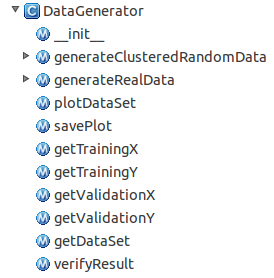
\includegraphics[width=0.4\textwidth]{img/GeneradorEsquema.png}
    \label{fig:EsquemaGenerador}
    \caption{Esquema general del generador de datos}
\end{figure}
Los dos métodos principales de estas clases y que son los encargados de generar y de obtener los conjuntos de datos serán explicados en detalle a continuación.

\subsection{Generación de datos aleatorios}
Tal como se ha descrito en secciones anteriores, en la implementación de la metaplasticidad propuesta por Diego Andina\citep{Andina2009}, la $fdp$ ($f_X(x)$) es fundamental y esto hace muy importante poder tener control sobre la distribución de probabilidad de los conjuntos de datos que se generan. Dado que se ha observado históricamente que las distribuciones gaussianas son las más comunes en los datos de origen natural, he utilizado para la generación de datos aleatorios la implementación que ofrece \textit{numpy} y que genera los datos siguiendo la siguiente función de distribución de probabilidad normal: 

\begin{center}
$pdf(x,\mu,\sigma) = \frac{1}{ \sigma \sqrt{2 \pi}} e^{\left(-\frac{{\left(\mu - x\right)}^{2}}{2 \, \sigma^{2}}\right)}$
\end{center}

El método, por tanto, construye el conjunto de datos en base a dos centroides aleatorios (que representan dos clases) etiquetando cada muestra en su clase. Dado lo compacto del código me decido a introducirlo en esta memoria para el lector interesado.
\begin{figure}[!h]{}
    \centering
    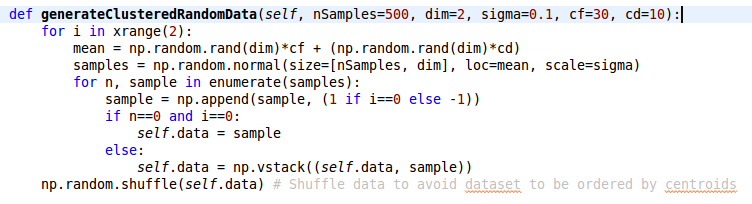
\includegraphics[width=0.8\textwidth]{img/generateClusteredRandomData.png}
    \label{fig:generateRandomMethod}
    \caption{Conjunto de datos con distribución normal}
\end{figure}

A continuación podemos ver un ejemplo del funcionamiento de la generación para 3 clases:
\begin{figure}[!h]{}
    \centering
    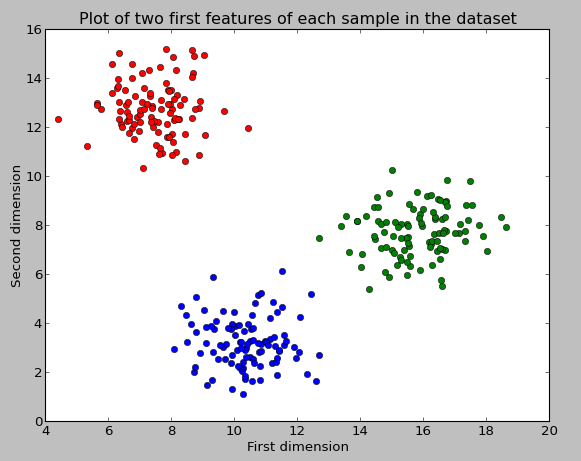
\includegraphics[width=0.4\textwidth]{img/clusteredData1.png}
    \label{fig:clusteredData1}
    \caption{Ejemplo de conjunto de datos generados aleatoriamente}
\end{figure}

\subsection{Obtención de datos reales}
Además de la experimentación con datos generados y con objeto de validar las propuestas, he implementado este segundo método en el generador de datos que se sirve de dos conjuntos de datos enormemente utilizados en el entrenamiento y verificación de sistemas de aprendizaje máquina y que son:
\begin{itemize}
	\item \href{https://archive.ics.uci.edu/ml/datasets/Breast+Cancer+Wisconsin+\%28Diagnostic\%29}{The Wisconsin Breast Cancer Data Set}
	\item \href{https://archive.ics.uci.edu/ml/datasets/Vertebral+Column}{Vertebral Column Data Set}
\end{itemize}

Una vez generados los datos, los métodos de obtención de los datos mantienen la misma interfaz independientemente del conjunto de datos con lo que sobre el mismo código de prueba, la elección del conjunto requiere tan solo la llamada de un método a otro.

\subsection{Implementación del generador de informes}
El generador de informes es un módulo compuesto de dos clases (\textit{LatexDocument} y \textit{LatexWriter}). 

(Diagrama de las clases)




\chapter{Experimentación}



\bibliographystyle{plain}
\bibliography{bibliography}

\end{document}
